\documentclass[aps,prb,showpacs,amsmath,amssymb,superscriptaddress]{revtex4-2}

\usepackage{tabularx}
\usepackage{bm}
%\usepackage[demo]{graphicx}
\usepackage{graphicx}

\usepackage{hyperref}
\hypersetup{colorlinks=true,urlcolor= blue,citecolor=blue,linkcolor= blue,bookmarks=true,bookmarksopen=false}

\usepackage{color}

\usepackage{amsmath,mathtools}
\usepackage{multirow}
\usepackage{dcolumn}
\usepackage{amssymb,amscd,xypic,bm,wasysym}
\usepackage{float}
\usepackage{cleveref}
\usepackage[caption=false,position=top,captionskip=0pt,farskip=0pt]{subfig}
\captionsetup[subfigure]{justification=raggedright,singlelinecheck=false}


\newcommand{\Red}[1]{\textcolor{red}{#1}}
\newcommand{\Blue}[1]{\textcolor{blue}{#1}}
%\newcommand{\vb}[1]{\boldsymbol{#1}}
\usepackage{soul}

% reset vec and hat style to a bold type
\let\oldhat\hat
\renewcommand{\hat}[1]{\oldhat{\mathbf{#1}}}
\renewcommand{\vec}[1]{\mathbf{#1}}
% stretches the vertical spacing of arrays/matrices
\renewcommand{\arraystretch}{1.5}
\setlength{\jot}{10pt}

\newcommand{\ham}{\mathcal{H}}
\newcommand{\cc}{c^{\dagger}}
\newcommand{\de}{\Delta}


\begin{document}

\title{Supplemental Material for ``Landau Level-like Topological Floquet Hamiltonians"}

\author{Aidan Winblad}
\affiliation{Department of Physics, Colorado State University, Fort Collins, CO 80523, USA}

\author{M. Tahir}
\affiliation{Department of Physics, Colorado State University, Fort Collins, CO 80523, USA}

\author{Hua Chen}
\affiliation{Department of Physics, Colorado State University, Fort Collins, CO 80523, USA}
\affiliation{School of Advanced Materials Discovery, Colorado State University, Fort Collins, CO 80523, USA}

\maketitle

\section{General framework of Floquet theory}\label{app:quantum-floquet-theory}

In this section we review the basic results of the Floquet theory and how to recast it into a matrix diagonalization problem. 
The discussion in this section is mostly following \cite{AEE}.

For a time-periodic Hamiltonian $H(t) = H(t+T)$ with period $T$, the time evolution of a wavefunction governed by it is described by the Schr\"{o}dinger equation
\begin{eqnarray}\label{eq:SchrHt}
	i\hbar \partial_t \psi(t) = H(t) \psi(t).
\end{eqnarray}
Floquet theorem states that $\psi(t)$ must satisfy
\begin{eqnarray}
	\psi(t+T) = \psi(t) e^{-i \frac{\epsilon T}{\hbar}},
\end{eqnarray}
where $\epsilon$ is a real number of energy units, or equivalently
\begin{eqnarray}
	\psi(t) = e^{-i \frac{\epsilon t}{\hbar}} u_{\epsilon}(t),
\end{eqnarray}
where $u_{\epsilon}(t) = u_{\epsilon}(t+T)$.

Here we give a proof that is closely analogous to Bloch theorem, based on plane wave expansion. An arbitrary wavefunction can be expanded into plane waves
\begin{eqnarray}
	\psi(t) = \sum_{\epsilon} c_\epsilon e^{-i \frac{\epsilon t}{\hbar}},
\end{eqnarray}
where $\epsilon\in \mathbb{R}$, while a time-periodic function $H(t)$ can only be written as a discrete Fourier series
\begin{eqnarray}
	H(t) = \sum_n H_n e^{i n \omega t},
\end{eqnarray}
where $\omega = 2\pi /T$, and $H_n = \frac{1}{T} \int_0^T H(t) e^{-i n \omega t} dt$. Substituting the two expansions above into Eq.~\ref{eq:SchrHt} gives
\begin{eqnarray}
	0 &=& \sum_\epsilon \left[ \sum_n H_n e^{-i \frac{(\epsilon - n \hbar \omega) t}{\hbar}} c_\epsilon - \epsilon c_\epsilon  e^{-i \frac{\epsilon t}{\hbar}} \right] \\\nonumber
	&=& \sum_\epsilon \left[ \sum_n H_n c_{\epsilon + n\hbar \omega} - \epsilon c_\epsilon  \right] e^{-i \frac{\epsilon t}{\hbar}},
\end{eqnarray}
which leads to
\begin{eqnarray}\label{eq:cepseqn}
	\sum_n H_n c_{\epsilon + n\hbar \omega} - \epsilon c_\epsilon = 0.
\end{eqnarray}
For an arbitrary $\epsilon\in \mathbb{R}$ we can define $\tilde{\epsilon} \in [-\hbar \omega /2, \hbar \omega /2)$ so that $\epsilon = \tilde{\epsilon} + m \hbar \omega$. It is apparent that Eq.~\ref{eq:cepseqn} only couples $c_{\tilde{\epsilon} + m\hbar \omega}$ belonging to the same $\tilde{\epsilon}$. We thus define
\begin{eqnarray}
	c_{\tilde{\epsilon} + m\hbar \omega} \equiv c_{m \tilde{\epsilon}},
\end{eqnarray}
so that Eq.~\ref{eq:cepseqn} becomes a set of coupled equations for $c_{m \tilde{\epsilon}}$, $m \in \mathbb{Z}$:
\begin{eqnarray}\label{eq:cepsteqn}
	\sum_n (H_n  - m\hbar \omega \delta_{n0} ) c_{m+n, \tilde{\epsilon}} = \tilde{\epsilon} c_{m \tilde{\epsilon}}.
\end{eqnarray}
Eq.~\ref{eq:cepseqn} is the eigenvalue problem of the infinite-dimensional matrix $\bar{Q}$ with the matrix elements
\begin{eqnarray}
	\bar{Q}_{m,m+n} = H_n - m \hbar \omega\delta_{n0},
\end{eqnarray}
which is also the quasienergy operator in \cite{AEE}. In practice the number of eigenvalues $\tilde{\epsilon}$ is determined by the dimension of $H(t)$. The solutions of Eq.~\ref{eq:SchrHt} are therefore
\begin{eqnarray}\label{eq:psitildee}
	\psi_{\tilde{\epsilon}} (t) = \sum_m c_{m \tilde{\epsilon}} e^{-i\frac{(\tilde{\epsilon} + m \hbar \omega)t}{\hbar}} = e^{-i\frac{\tilde{\epsilon} t}{\hbar}} \sum_m c_{m \tilde{\epsilon}} e^{-i m  \omega t} \equiv e^{-i\frac{\tilde{\epsilon} t}{\hbar}} u_{\tilde{\epsilon}}(t).
\end{eqnarray}

The proof above also gives a useful device for calculating the Floquet states $\psi_{\tilde{\epsilon}} (t) $ based on plane wave expansion. In general $H_n$ can be a complicated operator depending on, e.g. position, spin, etc., and $c_{m \tilde{\epsilon}}$ is a function depending on these quantum numbers. One can choose a representation that makes $H_0$ diagonal, such as the Bloch representation, leading to the eigenvalues $\epsilon_{n \bm k}$ of the time-averaged Hamiltonian ($H_0$). When $H_n$ is 0 for all $n \neq 0$, we have $\tilde{\epsilon} = \epsilon_{n \bm k} - m \hbar \omega$, $m \in \mathbb{Z}$. When $H_n$ is nonzero for any $n \neq 0$ there is in general no simple relationship between $\tilde{\epsilon}$ and $ \epsilon_{n \bm k}$. Nonetheless, when $H_n$, $n \neq 0$ can be viewed as perturbation the spectrum of $\tilde{\epsilon}$ is similar to that of $\epsilon_{n \bm k} - m \hbar \omega$, i.e., the eigenenergies $\epsilon_{n \bm k}$ together with infinite number of its copies shifted vertically by $m \hbar \omega$.

The importance of $\tilde{\epsilon}$ is that it completely determines the stroboscopic motion of an arbitrary Floquet wavefunction, i.e.,
\begin{eqnarray}
	\psi_{\tilde{\epsilon}} (t + m T) = e^{-i \frac{\tilde{\epsilon} m T}{\hbar}} \psi_{\tilde{\epsilon}} (t),\,\, \forall m\in \mathbb{Z}.
\end{eqnarray}
Since $\{\psi_{\tilde{\epsilon}}(t)\}$ is a complete set at time $t$, the stroboscopic evolution of an arbitrary wavefunction governed by $H(t)$ is
\begin{eqnarray}
	\Psi(t + m T) = \sum_{\tilde{\epsilon}} C_{\tilde{\epsilon}} e^{-i \frac{\tilde{\epsilon} m T}{\hbar}} \psi_{\tilde{\epsilon}} (t),
\end{eqnarray}
where $\Psi(t) =  \sum_{\tilde{\epsilon}} C_{\tilde{\epsilon}} \psi_{\tilde{\epsilon}} (t)$. The full time-evolution operator $\hat{U}(t_1,t_0)$ is therefore
\begin{eqnarray}\label{eq:Uevolve}
	\hat{U}(t_1,t_0) = \sum_{\tilde{\epsilon}}|\psi_{\tilde{\epsilon}} (t_1)\rangle \langle \psi_{\tilde{\epsilon}} (t_0) | = \sum_{\tilde{\epsilon}} |u_{\tilde{\epsilon}} (t_1)\rangle \langle u_{\tilde{\epsilon}} (t_0) | e^{-i\frac{\tilde{\epsilon}(t_1 - t_0)}{\hbar}}.
\end{eqnarray}
Now we introduce two operators
\begin{eqnarray}\label{eq:UFt1t0}
	\hat{U}^F(t_1,t_0) \equiv \sum_{\tilde{\epsilon}} |u_{\tilde{\epsilon}} (t_1)\rangle \langle u_{\tilde{\epsilon}} (t_0) |,
\end{eqnarray}
and
\begin{eqnarray}\label{eq:HFt0}
	\hat{H}^F_{t_0} \equiv \sum_{\tilde{\epsilon}} |u_{\tilde{\epsilon}} (t_0)\rangle\tilde{\epsilon} \langle u_{\tilde{\epsilon}} (t_0) |,
\end{eqnarray}
which allows us to rewrite Eq.~\ref{eq:Uevolve} as
\begin{eqnarray}
	\hat{U}(t_1,t_0) = \hat{U}_F(t_1,t_0) \exp\left[ -i\frac{(t_1 - t_0)\hat{H}^F_{t_0} }{\hbar}  \right] = \exp\left[ -i\frac{(t_1 - t_0)\hat{H}^F_{t_1} }{\hbar}  \right] \hat{U}_F(t_1,t_0).
\end{eqnarray}
Namely, the full time evolution is separated into two parts: $\hat{H}^F_{t_0}$ governs the stroboscopic evolution \emph{with the starting time} $t_0$, since
\begin{eqnarray}
	\exp\left[ -i\frac{m T \hat{H}^F_{t_0} }{\hbar}  \right] \psi_{\tilde{\epsilon}}(t_0) = e^{-i\frac{m T \tilde{\epsilon}}{\hbar} } \psi_{\tilde{\epsilon}}(t_0) = \psi_{\tilde{\epsilon}}(t_0 + m T),
\end{eqnarray}
while $\hat{U}_F (t_1, t_0)$ evolves the periodic part of the Floquet wavefunctions. $\hat{H}^F_{t_0} $ and $\hat{U}_F (t_1, t_0)$ are respectively called the Floquet Hamiltonian and the micromotion operator.

The most unsettling property of $\hat{H}^F_{t_0} $ is its dependence on $t_0$. To get rid of it we note that Eq.~\ref{eq:psitildee} implies
\begin{eqnarray}
	|u_{\tilde{\epsilon}}(t) \rangle =  \sum_{\alpha} \left(\sum_m c_{m \tilde{\epsilon}}^{\alpha} e^{-i m\omega t} \right)|\alpha\rangle \equiv\sum_\alpha  |\alpha\rangle U_{\alpha,\tilde{\epsilon}} (t) ,
\end{eqnarray}
where the time-independent basis $|\alpha\rangle$ spans the Hilbert space of $H(t)$, and $U (t)$ is a time-dependent unitary matrix satisfying $U(t+T) = U(t)$. Substituting this $|u_{\tilde{\epsilon}}(t) \rangle$ into Eq.~\ref{eq:SchrHt} gives
\begin{eqnarray}
	{\rm Diag}[\{\tilde{\epsilon}\}] = U^\dag H (t) U - i\hbar U^\dag \partial_t U = U^\dag \bar{Q} U,
\end{eqnarray}
where ${\rm Diag}[\{\tilde{\epsilon}\}]$ is a diagonal matrix with its eigenvalues being $\tilde{\epsilon}$. Comparing this with the effect of a time-dependent unitary transformation of the wavefunction $\psi' = U^\dag \psi$ in the Schr\"{o}dinger equation:
\begin{eqnarray}
	i\hbar \partial_t \psi' = (U^\dag H U - i\hbar U^\dag \partial_t U)\psi' \equiv H' \psi',
\end{eqnarray}
we can see that $U$ essentially transforms $H(t)$ to an effective Hamiltonian $H' = U^\dag \bar{Q}U$ which is time independent. The time evolution of $\psi$ can thus obtained as
\begin{eqnarray}
	\psi(t_1) &=& U(t_1) \psi'(t_1) = U(t_1) \exp\left[ -i \frac{H' (t_1 - t_0)}{\hbar}  \right] \psi'(t_0) \\\nonumber
	&=&  U(t_1) \exp\left[ -i \frac{H' (t_1 - t_0)}{\hbar}  \right] U^\dag(t_0) \psi(t_0)\\\nonumber
	&=&\hat{U}(t_1,t_0)\psi(t_0).
\end{eqnarray}
We therefore define
\begin{eqnarray}
	\hat{H}_F \equiv U^\dag \bar{Q} U = H'
\end{eqnarray}
as the Floquet effective Hamiltonian, which gives the time-evolution operator
\begin{eqnarray}\label{eq:Ut1t0}
	\hat{U}(t_1,t_0) =  U(t_1) \exp\left[ -i \frac{\hat{H}_F (t_1 - t_0)}{\hbar}  \right] U^\dag(t_0).
\end{eqnarray}
Intuitively, this means that the time evolution is obtained by first doing a gauge transformation to the time-independent gauge, evolving the system, and finally gauge-transforming back to the original gauge.

Although we have been assuming that $U(t)$ diagonalizes $\bar{Q}$, this is not necessary. Any time-independent unitary transformation multiplied to $U(t)$ can still make $\hat{H}_F$ time independent. To make connection between the $t_0$ dependent Floquet Hamiltonian $\hat{H}^F_{t_0}$ in Eq.~\ref{eq:HFt0} and the effective Hamiltonian $\hat{H}_F$, we use a minimal $U(t)$ that is independent of the basis of $\hat{H}(t)$:
\begin{eqnarray}
	U_F(t) =\sum_m c_m e^{-im\omega t},
\end{eqnarray}
which is a time-dependent scalar function. In the matrix form of $\bar{Q}$, this $U_F(t)$ block-diagonalizes $\bar{Q}$. All the diagonal blocks have the form $H_F - m\hbar \omega \bf{1}$. Here we removed the hat of $H_F$ to indicate that it is a matrix written in certain representation instead of an operator. In this particular representation or gauge, $|\alpha(t)\rangle = |\alpha\rangle U_F(t)$. We thus have
\begin{eqnarray}
	\hat{H}_{t_0}^F = \sum_{\tilde{\epsilon}}|u_{\tilde{\epsilon}}(t_0)\rangle \tilde{\epsilon} \langle u_{\tilde{\epsilon}} (t_0)| = \sum_{\alpha\beta} U_F(t_0) |\alpha\rangle (H_F)_{\alpha\beta} \langle \beta | U_F^\dag(t_0).
\end{eqnarray}
Or loosely speaking $\hat{H}_{t_0}^F =  U_F(t_0) \hat{H}_F U_F^\dag(t_0)$. Therefore the $t_0$ dependence in $\hat{H}_{t_0}^F$ is only due to a gauge transformation and is not physical. The complete information of time evolution can be obtained from $H_F$ \emph{and} $U_F$ according to Eq.~\ref{eq:Ut1t0}.

In practice, to obtain the quasienergy spectrum or $H_F$ we simply start from the eigenvalue problem Eq.~\ref{eq:cepseqn} for $\bar{Q}\equiv \bar{H} + \bar{Q}_0$, where $\bar{H}_{m,m+n} = H_n$ and $(\bar{Q}_0)_{m,m+n} = -m\hbar \omega \delta_{n0}$. We can either use perturbation theory and treat $\bar{H}$ as perturbation, which is accurate in the high-frequency limit, or directly diagonalize $\bar{Q}$ with a large enough cutoff. The first several terms in the perturbation series of $H_F$ are given in Eqs.~86-89 in \cite{AEE} ($m$ there should be $-m$ in our notation).

\section{High Frequency (Van Vleck) expansion from degenerate perturbation theory}

In order to understand the effects of coherent time-periodic modulation of quantum systems, we need an efficient method to obtain the Floquet
Hamiltonian $\hat{H}^{F}$ for a given time-dependent Hamiltonian $\hat{H} (\tau )$. Generally, for the Floquet systems, one would like to obtain a
suitable Hamiltonian $\hat{H}(\tau )$ given a desired static Hamiltonian $\hat{H}_{\rm eff}$. Usually the formal approach in making use of the
full eigenstates of a time-dependent model Hamiltonian is not feasible in practice. Therefore, one requires an approximate scheme that still provides
a valid description at least on the time-scales and energy-scales. Such an approach is provided by high-frequency approximations \cite{JHS,HSA,MGP,MBL,AEE,NGJ}.
Using the Van Vleck expansion within the degenerate perturbation theory as shown in Ref. \cite{AEE}, we can write the explicit expressions for the first few terms with $n=0,1,2$ as required;

\begin{eqnarray} \label{eq:44}
&&\hat{H}^{F(0)}=0,  \\
&&\hat{H}^{F(1)}=\hat{H}_{0},  \\
&&\hat{H}^{F(2)} =\sum_{m\neq 0}\frac{[\hat{H}_{m},\hat{H}_{-m}]}{m\hbar \omega }
\notag,\\
&&\hat{H}^{F(3)}={\displaystyle\sum_{m\neq0}}
\left(  \frac{[\hat{H}_{-m},[\hat{H}_{0},\hat{H}_{m}]]}{2(m\hbar\omega)^{2}
}+{\displaystyle\sum_{m^{\prime}\neq0,m}}
\frac{[\hat{H}_{-m^{\prime}},[\hat{H}_{m^{\prime}-m},\hat{H}_{m}
]]}{3mm^{\prime}(\hbar\omega)^{2}}\right)\notag.
\end{eqnarray}
Expressions for higher orders can be found in the above equations and refs. \cite{JHS,HSA,MGP,MBL,AEE,NGJ}. From a practical
point of view, and in the cases which we will be considering, one often engineers the time-dependent Hamiltonian in such a way that the approximate
Floquet Hamiltonian $\hat{H}_{\rm eff}$ =$\sum_{n=0}^{m}H^{F(n)}$ corresponds to the desired model Hamiltonian of the effective systems.

Some of the commutators are related by transpose or Hermitian conjugate.
As an example in $H^{F(2)}$ the transpose reduces the sum down by

\begin{align}
  \dfrac{[H_m,H_{-m}]}{m\hbar \omega} + \dfrac{[H_{-m}, H_m]}{-m\hbar\omega} &= \dfrac{[H_m,H_{-m}]}{m\hbar \omega} + \dfrac{[H_m, H_{-m}]}{m\hbar\omega} \\
  &= 2\dfrac{[H_m,H_{-m}]}{m\hbar \omega}
\end{align}
Additionally, an example in $H^{F(3)}$ the Hermitian conjugate reduces the sum down by

\begin{align}
  [H_{-m'},[H_{m'-m},H_m]]^{\dagger} &= [[H_{m'-m},H_m]^{\dagger}, H_{-m'}^{\dagger}] \nonumber \\
  &= [ [H_m^{\dagger}, H_{m'-m}^{\dagger}], H_{m'}] \nonumber \\
  &= [ [H_{-m}, H_{m-m'}], H_{m'}] \nonumber \\
  &= [H_{m'}, [H_{m-m'}, H_{-m}]]
\end{align}
or in general the following identity

\begin{equation}
  [A,[B,C]]^{\dagger} = [A^{\dagger}, [B^{\dagger}, C^{\dagger}]].
\end{equation}
With the symmetry in modes we have the following simplification

\begin{equation}
  \dfrac{[H_{-m'},[H_{m'-m},H_m]]}{mm'(\hbar\omega)^2} + \dfrac{[H_{m'},[H_{m-m'},H_{-m}]]}{(-m)(-m')(\hbar\omega)^2} = \dfrac{[H_{-m'},[H_{m'-m},H_m]] + h.c.}{mm'(\hbar\omega)^2}
\end{equation}

We can reduce the second and third perturbation summation terms to
\begin{align}
  H^{F(2)} &= \sum_{m> 0} \dfrac{2[H_m, H_{-m}]}{m\hbar\omega} \\
  H^{F(3)} &= \sum_{m> 0} \left( \dfrac{[H_{-m} , [H_0, H_m]] + h.c.}{2(m\hbar\omega)^2} + \sum_{m'\neq m} \dfrac{[H_{-m'}, [H_{m'-m}, H_m]] + h.c.}{3mm'(\hbar\omega)^2} \right)
\end{align}

\subsection{Non-uniform circularly polarized light on Dirac}
We start with the Dirac equation in 2D with a gauge potential

\begin{equation}
  \ham(t) = v_{F} \bm{\sigma} \cdot \left(\vec{p}+e\vec{A}(t)\right)
\end{equation}

where $\vec{A}(t) = \tfrac{E}{\omega} \langle -\sin{\omega t}, \tfrac{1}{2} \cos{(Kx)} \cos{(2\omega t)}$.
Which is made up of two electromagnetic wave sources.
The time dependent Hamiltonian becomes

\begin{equation}
  \ham(t) = v_{F} \left( \sigma_x \left(p_x - \dfrac{f}{\omega} \sin{\omega t} \right) + \sigma_y \left(p_y + \dfrac{f}{2\omega} \cos{(Kx)} \cos{(2\omega t)} \right) \right),
\end{equation}
where $f = eE$.
Performing the Fourier time-transform from

\begin{equation}
  H_n = \dfrac{1}{T} \int_{0}^{T} \ham(t) e^{-in\omega t} dt
\end{equation}
gives the following terms

\begin{align}
  H_0 &= v_{F} \bm{\sigma}\cdot \vec{p} \\
  H_{\pm1} &= \pm \sigma_x \dfrac{i v_{F} f}{2\omega} \\
  H_{\pm2} &= \sigma_y \dfrac{v_{F} f}{4\omega} \cos{(Kx)}.
\end{align}

We compute the following Hermitian commutators for the high-frequency expansion

\begin{align}
  &[H_{1}, H_{-1}] \\
  &[H_{2}, H_{-2}] \\
  &[H_{-1}, [H_{0}, H_{1}]] \\
  &[H_{-2}, [H_{0}, H_{2}]] \\
  &[H_{1}, [H_{-2}, H_{1}]] \\
  &[H_{-1}, [H_{-1}, H_{2}]].
\end{align}
We find each term to be

\begin{equation}
  [H_{1}, H_{-1}] = [H_{2}, H_{-2}] = 0
\end{equation}

\begin{align}
  [H_{0}, H_{\pm1}] &= \pm \sigma_z \dfrac{v_{F}^{2} f}{\omega} p_y \nonumber \\
  [H_{1}, [H_{0}, H_{-1}]] &= - \sigma_y \dfrac{v_{F}^3 f^2}{\omega^2} p_y \\
  [H_{0}, H_{\pm2}] &= \pm i \sigma_z \dfrac{v_{F}^{2} f}{4\omega} \left(p_x \cos{(Kx)} + \cos{(Kx)} p_x \right) \nonumber \\
  [H_{2}, [H_{0}, H_{-2}]] &= - \sigma_y \dfrac{v_{F}^3 f^2}{2 \omega^2} \left( p_x \cos^2{(Kx)} + \cos^2{(Kx)} p_x \right) \\
  [H_{\pm1}, H_{2}] &= \mp \sigma_z \left(\dfrac{v_{F} f}{2\omega} \right)^{2} \cos{(Kx)} \nonumber \\
  [H_{1}, [H_{-2},H_{-1}]] &=
\end{align}

\subsection{Non-uniform circularly polarized light on 2DEG} \label{fll-2deg-derivation}

We start with the Schrodinger equation in 2D with a gauge potential field

\begin{equation}
  \ham(t) = \dfrac{\left(\vec{p} + e\vec{A}(t) \right)^2}{2m^*}
\end{equation}
where $\vec{A}(t) = \tfrac{E}{\omega} \langle -\sin{\omega t} , \cos{(Kx)}\cos{\omega t} \rangle$.
Which is made up of two electromagnetic wave sources.
The time dependent Hamiltonian becomes

\begin{equation}
\begin{split}
  \ham(t) = &\dfrac{1}{2m^*} \Big[ p_x^2 + p_y^2 + \dfrac{e^2 E^2}{2\omega^2}(1+\cos^2{(Kx)}) + \dfrac{e^2 E^2}{2\omega^2}\sin^2{(Kx)} \cos{2\omega t} \\
  &+ \dfrac{2eE}{\omega} p_y \cos{(Kx)} \cos{\omega t} - \dfrac{2eE}{\omega} p_x \sin{\omega t} \Big]
\end{split}
\end{equation}

Performing the Fourier time-transform from

\begin{equation}
  H_n = \dfrac{1}{T} \int_{0}^{T} \ham(t) e^{-in\omega t} dt
\end{equation}
gives the following terms

\begin{align}
  H_0 &= \dfrac{1}{2m^*} \left( p_x^2 + p_y^2 + \dfrac{e^2 E^2}{2 \omega^2} (1+\cos^2{(Kx)}) \right) \\
  H_{\pm1} &= \dfrac{1}{2m^*} \dfrac{eE}{\omega}\left( \pm i p_x + p_y \cos{(Kx)} \right) \\
  H_{\pm2} &= -\dfrac{1}{2m^*} \dfrac{e^2 E^2}{4\omega^2} \sin^2{(Kx)}
\end{align}

We compute the following Hermitian commutators for the high-frequency expansion

\begin{align}
  [H_{1}, H_{-1}] &= -\dfrac{1}{2m^*} \dfrac{\hbar K e^2 E^2}{\omega^2} p_y \sin{(Kx)} \\
  [H_{2}, H_{-2}] &= 0
\end{align}
then

\begin{equation}
  H^{F(2)} = \dfrac{2[H_{1}, H_{-1}]}{\hbar \omega} = -\dfrac{1}{2m^*} \dfrac{2 K e^2 E^2}{\omega^3} p_y \sin{(Kx)} \\
\end{equation}
The full Hamiltonian to first order in $\hbar \omega$ becomes

\begin{equation}
  H_{\text{eff}} &= \dfrac{1}{2m^*} \left( p_x^2 + p_y^2 + \dfrac{e^2 E^2}{2 \omega^2} (1+\cos^2{(Kx)}) - \dfrac{2 K e^2 E^2}{\omega^3} p_y \sin{(Kx)} \right).
\end{equation}
We can further manipulate by shifting the energy by a constant and completing the square w.r.t. $p_y$ and $\sin{(Kx)}$ terms to get
\begin{equation}
  H_{\text{eff}} &= \dfrac{1}{2m^*} \left( p_x^2 + \left(p_y - \dfrac{ K e^2 E^2}{m^*\omega^3} \sin{(Kx)}\right)^2 + \dfrac{e^2 E^2}{2 \omega^2} \cos^2{(Kx)} - \dfrac{K^2 e^4 E^4}{m^{*2}\omega^6} \sin^2{(Kx)} \right).
\end{equation}

\section{Tight-binding model Dirac}\label{app:tbm-dirac}

We start with a nearest-neighbor single-orbital tight-binding Hamiltonian

\begin{equation}
  \ham = - \sum_{jl\alpha,j'l'\beta} h \cc_{jl\alpha} c_{j'l'\beta} + h.c.
\end{equation}
The incident laser beam in vector potential forms looks like

\begin{equation} \label{eq:AvecDirac}
  \vec{A}(\vec{r},t) = \dfrac{E}{\omega} \langle -\sin \omega t, \dfrac{1}{2} \sin(Kx) \cos 2\omega t \rangle.
\end{equation}
Using the following approximation for smoothly varying vector potential fields

\begin{equation}
  \int_{\vec{r}_{j,l}^{\alpha}} ^{\vec{r}_{j',l'}^{\beta}} \vec{A}(\vec{r},t) \cdot d\vec{l} \approx \vec{A} \left( \dfrac{ \vec{r}_{j',l'}^{\beta} + \vec{r}_{j,l}^{\alpha} }{2}, t \right) \cdot \left( \vec{r}_{j',l'}^{\beta} - \vec{r}_{j,l}^{\alpha} \right)
\end{equation}


where

\begin{align}
  \vec{a}_1 &= \sqrt{3}a\hat{x} \\
  \vec{a}_2 &= 3a\hat{y} \\
  \vec{r}_{jl}^{A_1} &= j\vec{a}_1 + l\vec{a}_2 \\
  \vec{r}_{jl}^{B_1} &= (j+\tfrac{1}{2})\vec{a}_1 + (l+\tfrac{1}{6})\vec{a}_2 \\
  \vec{r}_{jl}^{A_2} &= (j+\tfrac{1}{2})\vec{a}_1 + (l+\tfrac{1}{2})\vec{a}_2 \\
  \vec{r}_{jl}^{B_2} &= (j+1)\vec{a}_1 + (l+\tfrac{2}{3})\vec{a}_2.
\end{align}

\begin{figure}[h]
  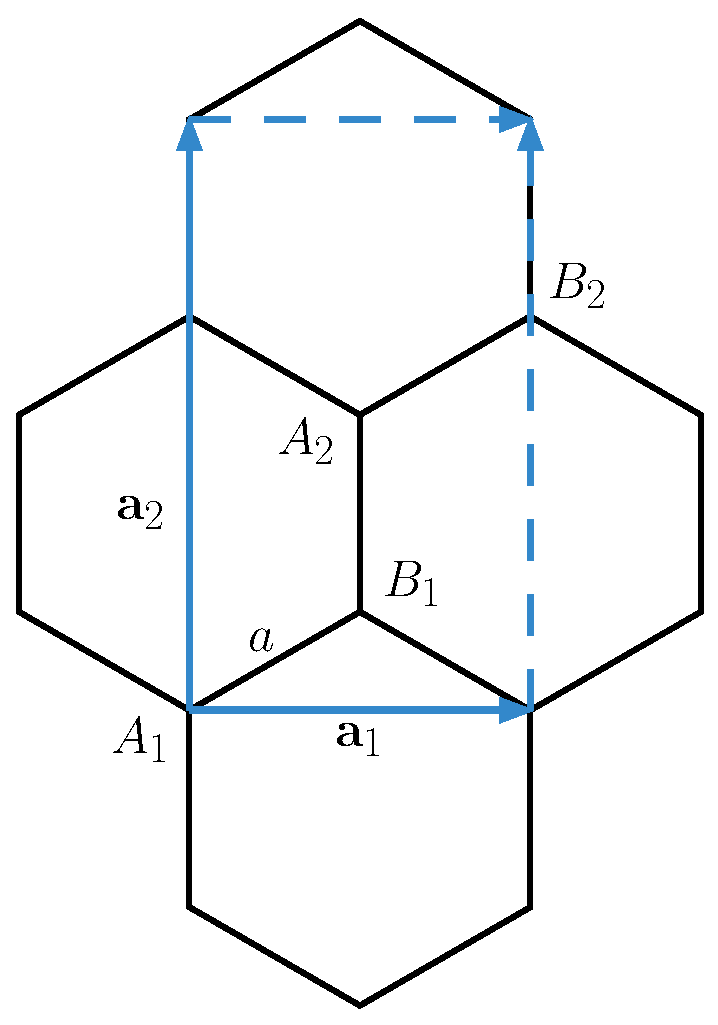
\includegraphics[width=0.30\textwidth]{./dirac-floquet-unit-cell.pdf}
\caption{Unit cell for dirac system with gauge potential with tranlation symmetry in the $y-axis$ described by Eq.~\eqref{eq:AvecDirac}.}
  \label{fig:dirac-floquet-unit-cell}
\end{figure}
Applying a Peierls substitution the Hamiltonian becomes

\begin{equation}
\begin{split}
  \ham (t) = -\sum_{jl} \ &h_{jlA_1}^{jlB_1}(t) \cc_{jlA_1} c_{jlB_1} + h_{jlB_1}^{jlA_2}(t) \cc_{jlB_1} c_{jlA_2} + h_{jlA_2}^{jlB_2}(t) \cc_{jlA_2} c_{jlB_2} \\
      + &h_{jlB_1}^{j+1,lA_1}(t) \cc_{jlB_1} c_{j+1,lA_1} + h_{jlB_2}^{j+1,l,A_2} \cc_{jlB_2} c_{j+1,lA_2}(t) \\
      + &h_{jlB_2}^{j+1,l+1,A_1}(t) \cc_{jlB_2} c_{j+1,l+1,A_1} + h.c.
\end{split}
\end{equation}
where in general

\begin{equation}
  h_{jl\alpha}^{j'l'\beta} (t) \approx h \exp \left[ i \phi_0 \left(-\dfrac{x_{j'l'}^{\beta} - x_{jl}^{\alpha}}{a} \sin\omega t + \dfrac{y_{j'l'}^{\beta} - y_{jl}^{\alpha}}{2a} \cos\left(K \dfrac{x_{j'l'}^{\beta} + x_{jl}^{\alpha}}{2}\right) \cos 2\omega t \right) \right],
\end{equation}
where $\phi_{0} = eE/(\hbar \omega)$.
More explicitly for each term

\begin{align}
  h_{jlA_1}^{jlB_1}(t) &\approx h \exp \left[ i\phi_0 \left(-\dfrac{\sqrt{3}}{2} \sin\omega t + \dfrac{1}{4} \sin(\sqrt{3}Ka(j+\tfrac{1}{4})) \cos 2\omega t \right) \right] \\
  h_{jlB_1}^{jlA_2}(t) &\approx h \exp \left[ i\phi_0 \left(\dfrac{1}{2} \sin(\sqrt{3}Ka(j+\tfrac{1}{2})) \cos 2\omega t \right) \right] \\
  h_{jlA_2}^{jlB_2}(t) &\approx h \exp \left[ i\phi_0 \left(-\dfrac{\sqrt{3}}{2} \sin\omega t + \dfrac{1}{4} \sin(\sqrt{3}Ka(j+\tfrac{3}{4})) \cos 2\omega t \right) \right]
\end{align}
\begin{align}
  h_{jlB_1}^{j+1,lA_1}(t) &\approx h \exp \left[ i\phi_0 \left(-\dfrac{\sqrt{3}}{2} \sin\omega t - \dfrac{1}{4} \sin(\sqrt{3}Ka(j+\tfrac{3}{4})) \cos 2\omega t \right) \right] \\
  h_{jlB_2}^{j+1,lA_2}(t) &\approx h \exp \left[ i\phi_0 \left(-\dfrac{\sqrt{3}}{2}\sin\omega t -\dfrac{1}{4} \sin(\sqrt{3}Ka(j+\tfrac{5}{4})) \cos 2\omega t \right) \right] \\
  h_{jlB_2}^{j+1,l+1,A_1}(t) &\approx h \exp \left[ i\phi_0 \left(\dfrac{1}{2} \sin(\sqrt{3}Ka(j+1)) \cos 2\omega t \right) \right]
\end{align}

The incident laser beam allows for translation symmetry along the y-axis, so we can reduce the dimension of the Hamiltonian with the following Fourier transform

\begin{equation}
  \cc_{jl\alpha} = \dfrac{1}{N_y} \sum_k \cc_{jk\alpha} e^{ik\hat{y}\cdot\vec{R_l}} = \dfrac{1}{N_y} \sum_k \cc_{jk\alpha} e^{ik(3la)}
\end{equation}
The Hamiltonian then becomes

\begin{equation}
\begin{split}
  \ham (t) = -\sum_{jk} \ &h_{jlA_1}^{jlB_1}(t) \cc_{jkA_1} c_{jkB_1} + h_{jlB_1}^{jlA_2}(t) \cc_{jkB_1} c_{jkA_2} + h_{jlA_2}^{jlB_2}(t) \cc_{jkA_2} c_{jkB_2} \\
      + &h_{jlB_1}^{j+1,lA_1}(t) \cc_{jkB_1} c_{j+1,kA_1} + h_{jlB_2}^{j+1,l,A_2} \cc_{jkB_2} c_{j+1,kA_2}(t) \\
      + &h_{jlB_2}^{j+1,l+1,A_1}(t) e^{-i3ka} \cc_{jkB_2} c_{j+1,kA_1} + h.c.
\end{split}
\end{equation}

Making use of Floquet theory we can make the Hamiltonian time-independent with the following time domain Fourier transform

\begin{equation}
  H_{ab,n,k} = \dfrac{1}{2\pi} \int_0^{2\pi} \ham_{ab}(k,t) e^{-in\tau} d\tau
\end{equation}
where $a,b$ represent the matrix indes of the previous Hamiltonian and $n$ is the $n$-th order mode of light.
Each term has the general following form

\begin{equation}
  H_{ab,n,k} = \dfrac{1}{2\pi} \int_0^{2\pi} e^{i Z_1 \sin\tau + i Z_2 \cos2\tau - in\tau} d\tau
\end{equation}
which looks a lot like the Hansen-Bessel integral function.
However, because of the linear combination of $\sin\tau$ and $\cos 2\tau$, there is no elementary solution to the integral as currently defined.
We thus solve the integral numerically for each given $n$.
After the time domain Fourier transform the Hamiltonian can be reduced to the following matrix form
\begin{equation}
  H_n = -\sum_{jk} \left[ \Psi_{jk}^{\dagger} H_{jj} \Psi_{jk} + \Psi_{jk}^{\dagger} H_{j,j+1,k}' \Psi_{j+1,k} + h.c. \right]
\end{equation}

\[
  H_{j,j} =
  \begin{bmatrix}
    0 & 0 & 0 & 0 \\
    h^{jlA_1}_{jlB_1} & 0 & 0 & 0 \\
    0 & h^{jlB_1}_{jlA_2} & 0 & 0 \\
    0 & 0 & h^{jlA_2}_{jlB_2} & 0 \\
  \end{bmatrix}
\]
and
\[
  H'_{j,j+,k} =
  \begin{bmatrix}
    0 & h^{j+1,lA_1}_{jlB_1} & 0 & h^{j+1,l+1,A_1}_{jlB_2} e^{i\vec{k}\cdot\vec{a}_2} \\
    0 & 0 & 0 & 0 \\
    0 & 0 & 0 & h^{j+1,lA_2}_{jlB_2} \\
    0 & 0 & 0 & 0
  \end{bmatrix},
\]
with $\vec{k} = k\hat{y}$ and $\Psi_{jk} = [c_{jkA_1}, c_{jkB_1}, c_{jkA_2}, c_{jkB_2}]^T$.

The quasienergy energy matrix has elements $Q_{m,m+n} = H_n - m\hbar\omega\delta_{n0}$.
We choose a cutoff for mode $m$, $|m|\leq m_c$, where $m_c$ is a positive integer.
This cuts the matrix down to have $N_m = 2m_c+1$ diagonal blocks, where each block is of size a $N_S = 2r_c +1$ square matrix, $H_n$, and $r_c$ is the cutoff radius of unit cells.
The matrix can be solved using an eigenvalue solver, producing $N_m N_S$ eigenenergies and eigenvectors for a given electric field strength $E$.
It is difficult to glean any information from looking at all the energies but one can do a projection to the $m=0$ mode to highlight which energies belong to it.
This is still not all that imformative because when using a finite system we discretize the brillouin zone uniformly and it does not necessarily mean we are picking energy values close to the folded in Dirac point, since the unperturbed brillouin zone gets folded into the perturbed smaller brillouin zone.

\section{Tight-binding model 2DEG}

We start with a nearest-neighbor single-orbital tight-binding Hamiltonian on a square lattice

\begin{equation}
  \ham = \sum_{j,l} -h (\cc_{j,l} c_{j+1,l} + \cc_{j,l} c_{j,l+1} + h.c.)
\end{equation}
The incident laser beam as a vector potential is as follows

\begin{equation}
  \vec{A}(\vec{r}, t) = \dfrac{E}{\omega} \langle -\sin\omega t, \cos(Kx) \cos\omega t \rangle.
\end{equation}
Using the following approximation for smoothly varying vector potential fields

\begin{equation}
  \int_{\vec{r}_a}^{\vec{r}_b} \vec{A}(\vec{r},t) \cdot d\vec{l} \approx \vec{A} \left( \dfrac{\vec{r}_b+\vec{r}_b}{2}, t \right) \cdot (\vec{r}_b - \vec{r}_a)
\end{equation}
and using Peierls substitution the Hamiltonian becomes

\begin{equation}
  \ham(t) = -\sum_{j,l} (h_{j,j+1}(t) \cc_{j,l} c_{j+1,l} + h_{l,l+1}(t) \cc_{j,l} c_{j,l+1} + h.c.),
\end{equation}
where

\begin{align}
  h_{j,j+1}(t) &\approx h \exp\left(-i \dfrac{eEa}{\hbar \omega} \dfrac{x_{j+1}-x_j}{a} \sin \omega t\right) \nonumber \\
  &= h \exp\left(-i \phi_0 \sin \omega t\right) \\
  h_{l,l+1}(t) &\approx h \exp\left(i \dfrac{eEa}{\hbar \omega} \dfrac{y_{l+1}-y_l}{a} \cos(Kx_j)\cos \omega t\right) \nonumber \\
  &= h \exp\left(i \phi_0 \cos(Kx_j)\cos \omega t\right).
\end{align}

The incident laser beam allows for translation symmetry along the y-axis, so we can reduce the dimension of the Hamiltonian with the following Fourier transform

\begin{equation}
  \cc_{j,l} = \dfrac{1}{\sqrt{N_y}} \sum_k \cc_{j,k} e^{ik\hat{y}\cdot \vec{r}_{l}} = \dfrac{1}{\sqrt{N_y}} \sum_k \cc_{j,k} e^{ikla}.
\end{equation}
The Hamiltonian then becomes

\begin{align}
  \ham(t) &= \sum_{j,k} ( h_{l,l+1}(t) e^{-ika} + h_{l,l+1}^*(t) e^{ika}) \cc_{j,k} c_{j,k} + (h_{j,j+1}(t) \cc_{j,k} c_{j+1,k} + h.c.) \\
  &= \sum_{j,k} 2h\cos( \phi_0 \cos(Kx_j) \cos \omega t - ka ) \cc_{j,k} c_{j,k} + (h e^{i\phi_0 \sin \omega t} \cc_{j,k} c_{j+1,k} + h.c.).
\end{align}
Making use of Floquet theory we can make the Hamiltonian time-independent with the following time Fourier transform

\begin{align}
  \ham_{ab,n}(k) &= \dfrac{1}{T} \int_0^T \ham_{ab}(k,t) e^{-in \omega t} dt \\
  &= \dfrac{1}{2\pi} \int_0^{2\pi} \ham_{ab}(k,t) e^{-in\tau} d\tau
\end{align}
where $a,b$ represent the matrix index of the previous Hamiltonian and $n$ is the $n$-th order mode of light.
We will make use of the following Hansen-Bessel integral formulas

\begin{equation} \label{eq: hansen-bessel}
  J_n(z) = \dfrac{1}{2\pi} \int_0^{2\pi} e^{in\tau - z \sin\tau} d\tau = \dfrac{1}{2\pi} \int_0^{2\pi} e^{in\tau - in\pi/2 + z\cos\tau} d\tau,
\end{equation}
note that the integral bound can be the same due to the integrand being periodic from $[0,2\pi]$.
Recall, Bessel function identities for $n \in \mathbb{Z}$

\begin{align}
  J_n(-z) = (-1)^n J_n(z) \\
  J_{-n}(z) = (-1)^n J_n(z)
\end{align}
The terms for given $k$ become the following time Fourier transforms

\begin{align}
  \ham_{j,j,n}(k) &= -\dfrac{h}{2\pi} \int_0^{2\pi} \left( e^{i \phi_0 \cos(Kx_j) \cos \tau - ika - in\tau} + e^{-i \phi_0 \cos(Kx_j) \cos \tau + ika - in\tau} \right) d\tau \nonumber \\
    &= -h \left( \dfrac{e^{-ika}}{2\pi} \int_0^{2\pi} e^{i z \cos \tau - in\tau} d\tau + \dfrac{e^{ika}}{2\pi} \int_0^{2\pi} e^{-i z \cos \tau - in\tau} d\tau \right) \nonumber \\
    &= -h \left( \dfrac{e^{-ika -in\pi/2}}{2\pi} \int_0^{2\pi} e^{i z \cos \tau - in\tau + in\pi/2} d\tau + \dfrac{e^{ika - in\pi/2}}{2\pi} \int_0^{2\pi} e^{-i z \cos \tau - in\tau + in\pi/2} d\tau \right) \nonumber \\
    &= -h e^{-in\pi/2} \left( J_{-n}(z) e^{-ika} + J_{-n}(-z) e^{ika} \right) \nonumber \\
    &= -h J_n(z) e^{-in\pi/2} ( e^{ika} +  e^{-ika+in\pi} ) \nonumber \\
    &= -h J_n(z) ( e^{i(ka-n\pi/2)} +  e^{-i(ka-n\pi/2)} ) \nonumber \\
    &= -2h J_n(\phi_0 \cos(Kx_j)) \cos \left( ka -n\pi/2 \right)
\end{align}
and

\begin{align}
  \ham_{j,j+1,n} &= -\dfrac{h}{2\pi} \int_0^{2\pi} e^{-i \phi_0 \sin \tau - in\tau} d\tau \nonumber \\
  &= -h J_{-n}(\phi_0) \nonumber \\
  &= -h (-1)^n J_n(\phi_0) \\
  \ham_{j+1,j,n} &= -\dfrac{h}{2\pi} \int_0^{2\pi} e^{i \phi_0 \sin \tau - in\tau} d\tau \nonumber \\
    &= -h J_{-n}(-\phi_0) \nonumber \\
    &= -h J_n(\phi_0)
\end{align}

This completes finding all the matrix terms for the quasienergy matrix $\bar{Q}$ for a 2DEG tight binding model with incident inhomogeneous laser light.




\section{Chern number of Landau levels}
In this section we discuss how to understand the Chern number of Landau levels. For two-dimensional periodic systems, the 2D Brillouin zone is a closed manifold, and one can define the Chern number as a topological invariant for the mapping between complex functions (ground state wavefunctions) and this manifold. However, for Landau levels the system does not have translational symmetry which causes a conceptual difficulty in defining Chern numbers.

To address this difficulty, let us start from the Chern number of typical 2D Bloch Hamiltonians. The Berry curvature of band $n$ at crystal momentum $\mathbf k$ is defined as
\begin{eqnarray}\label{eq:Berrycurv}
	\Omega_{n\mathbf k} = \hat{z}\cdot (\nabla_{\mathbf k} \times \mathbf A_{n \mathbf k})= \hat z\cdot (\nabla_{\mathbf k} \times \langle u_{n \mathbf k} | i\nabla_{\mathbf k} | u_{n \mathbf k}\rangle )
\end{eqnarray}
The Chern number for band $n$, which must not touch other bands throughout the Brillouin zone, is defined as
\begin{eqnarray}
	C_{n} = \int \frac{d^2\mathbf k}{2\pi} \Omega_{n \mathbf k}
\end{eqnarray}
However, according to Eq.~\eqref{eq:Berrycurv}, $C_n$ can be rewritten into
\begin{eqnarray}
	C_{n} &=&\int \frac{d^2\mathbf k}{2\pi} \partial_{k_x} \langle u_{n \mathbf k}| i\partial_{k_y} | u_{n \mathbf k}\rangle  - \int \frac{d^2\mathbf k}{2\pi} \partial_{k_y} \langle u_{n \mathbf k}| i\partial_{k_x} | u_{n \mathbf k}\rangle \\\nonumber
	&=&\frac{1}{2\pi}\int d{k_x}\partial_{k_x}\int dk_y  \langle u_{n \mathbf k}| i\partial_{k_y} | u_{n \mathbf k}\rangle - \frac{1}{2\pi}\int d{k_y}\partial_{k_y}\int dk_x  \langle u_{n \mathbf k}| i\partial_{k_x} | u_{n \mathbf k}\rangle
\end{eqnarray}
It is worth noting that the last result is related to the expectation value of polarization (or position operator) in a Bloch state:
\begin{eqnarray}
	 \langle n\mathbf k | \mathbf r | n' \mathbf k'\rangle &=& \int d^2\mathbf r \psi_{n'\mathbf k'}^\dag (\mathbf r) \mathbf r \psi_{n \mathbf k} (\mathbf r) \\\nonumber
	 & =& \int d^2\mathbf r u_{n\mathbf k}^\dag (\mathbf r) e^{-i\mathbf k \cdot \mathbf r}\mathbf r e^{i\mathbf k'\cdot \mathbf r } u_{n' \mathbf k'} (\mathbf r) \\\nonumber
	 &=& \int d^2\mathbf r u_{n\mathbf k}^\dag (\mathbf r) e^{-i\mathbf k \cdot \mathbf r}\mathbf (-i\partial_{\mathbf k'} e^{i\mathbf k'\cdot \mathbf r }) u_{n' \mathbf k'} (\mathbf r)\\\nonumber
	 &=& -i\partial_{\mathbf k'} \langle n\mathbf k | n'\mathbf k'\rangle  + \int d^2\mathbf r u_{n\mathbf k}^\dag (\mathbf r) e^{-i\mathbf k \cdot \mathbf r}e^{i\mathbf k'\cdot \mathbf r }  \left[i\partial_{\mathbf k'} u_{n' \mathbf k'} (\mathbf r)\right] \\\nonumber
	 &=&  -i\delta_{nn'} \frac{(2\pi)^2}{V_{\rm uc}}\partial_{\mathbf k'}\delta(\mathbf k  - \mathbf k')   + \int d^2\mathbf r u_{n\mathbf k}^\dag (\mathbf r) e^{-i\mathbf k \cdot \mathbf r}e^{i\mathbf k'\cdot \mathbf r }  \left[i\partial_{\mathbf k'} u_{n' \mathbf k'} (\mathbf r)\right] \\\nonumber
	 &=&  -i\delta_{nn'} \frac{(2\pi)^2}{V_{\rm uc}}\partial_{\mathbf k'}\delta(\mathbf k  - \mathbf k')   + \sum_{\mathbf R}\int_{\rm uc}  d^2\mathbf r u_{n\mathbf k}^\dag (\mathbf r) e^{i(\mathbf k' - \mathbf k) \cdot \mathbf r} \left[i\partial_{\mathbf k'} u_{n' \mathbf k'} (\mathbf r)\right] e^{i(\mathbf k' - \mathbf k)\cdot \mathbf R} \\\nonumber
	 &=& -i\delta_{nn'} \frac{(2\pi)^2}{V_{\rm uc}}\partial_{\mathbf k'}\delta(\mathbf k  - \mathbf k')   + \frac{(2\pi)^2}{V_{\rm uc}} \delta(\mathbf k - \mathbf k') \int_{\rm uc}  d^2\mathbf r u_{n\mathbf k}^\dag (\mathbf r) \left[i\partial_{\mathbf k'} u_{n' \mathbf k'} (\mathbf r)\right] e^{i(\mathbf k' - \mathbf k)\cdot \mathbf R}\\\nonumber
	 &=& \frac{(2\pi)^2}{V_{\rm uc}} \left[i\delta_{nn'} \partial_{\mathbf k}\delta(\mathbf k - \mathbf k') + \langle u_{n \mathbf k} | i\partial_{\mathbf k} | u_{n'\mathbf k}\rangle \delta(\mathbf k-\mathbf k') \right]
\end{eqnarray}
where we have used the normalization condition of 2D Bloch states $\langle n\mathbf k | n'\mathbf k'\rangle = \delta_{nn'} \frac{(2\pi)^2}{V_{\rm uc}}\delta(\mathbf k  - \mathbf k')  $ with $V_{\rm uc}$ the unit cell volume or area. The above result means that
\begin{eqnarray}
	\frac{a_y}{2\pi} \int d k_y \langle n\mathbf k | \mathbf r | n\mathbf k\rangle &\equiv& N \mathbf r_{n} (k_x) = \frac{a_y}{2\pi} \int d k_y \lim_{\mathbf k'\rightarrow \mathbf k} \langle n\mathbf k | \mathbf r | n\mathbf k'\rangle \\\nonumber
	&=& \frac{a_y}{2\pi} N \int dk_y \langle u_{n\mathbf k}| i\partial_{\mathbf k} |u_{n \mathbf k}\rangle
\end{eqnarray}
where $a_y$ is the lattice constant along $y$. Namely
\begin{eqnarray}\label{eq:intdkyA}
\frac{1}{2\pi} \int dk_y \langle u_{n\mathbf k}| i\partial_{\mathbf k} |u_{n \mathbf k}\rangle = \frac{\mathbf r_n(k_x)}{a_y}.
\end{eqnarray}
Therefore
\begin{eqnarray}\label{eq:Cnpump}
	C_n &=& \frac{1}{a_y} \int dk_x \partial_{k_x} y_n(k_x) - \frac{1}{a_x} \int dk_y \partial_{k_y} x_n(k_y) \\\nonumber
	&=& \frac{1}{a_y} \left[y_n|_{k_x = \frac{2\pi}{a_x}} - y_n|_{k_x = 0} \right] -  \frac{1}{a_x} \left[x_n|_{k_y = \frac{2\pi}{a_x}} - x_n|_{k_y = 0} \right] \\\nonumber
	&\equiv &\frac{\Delta y_n}{a_y} - \frac{\Delta x_n}{a_x}
\end{eqnarray}
In other words, the Chern number can be understood as an effect of adiabatic pumping. The parameter defining the pump is $k_x$ (1st term in the above equation) or $k_y$ (2nd term in the above equation). When the pumping parameter increases by a period, the expectation value of the position operator $y_n$ (or $x_n$) for the given band does not necessarily return to itself. A nonzero change leads to the finite Chern number. A caveat that is not mentioned in many references or textbooks is that since $\mathbf{A}_{n\mathbf k}$ is not a gauge invariant quantity, the two individual terms in the last line of Eq.~\eqref{eq:Cnpump} are not separately well defined. Instead, one can choose a gauge so that $A_x(k_y = 0) = A_{x}(k_y = \frac{2\pi}{a_y})$ [but $A_y(k_x = 0) \neq A_{y}(k_x = \frac{2\pi}{a_x})$, since otherwise $C_n$ always vanishes], so that
\begin{eqnarray}
	C_n = \frac{\Delta y_n}{a_y},~ A_x\left(k_y + \frac{2\pi}{a_y}\right) = A_x(k_y)
\end{eqnarray}
In this manner, the Chern number is equivalent to the change of the $y$-component of the center-of-mass position of the given Bloch state, when $k_x$ changes by $2\pi/a_x$.

The above adiabatic pumping understanding of the Chern number can now be used to define the Chern number of Landau levels, for which the Hamiltonian can only be made translation invariant along one direction. The Landau level Hamiltonian for a uniform magnetic field $B\hat{z} = \nabla \times (Bx\hat{y}) = \nabla \times \mathbf A$ is
\begin{eqnarray}
	H = \frac{p_x^2}{2 m } + \frac{(p_y + eBx)^2}{2m}
\end{eqnarray}
Assuming the eigenfunctions are $\psi(x,y)$, we can first make use of the translation symmetry along $y$ to define
\begin{eqnarray}
	\psi(x,y) = \frac{1}{2\pi}\int dk \phi(x,k) e^{iky}
\end{eqnarray}
The inverse transform is
\begin{eqnarray}
\psi(x,k) = \int dy \psi(x,y) e^{-iky}
\end{eqnarray}
which is consistent with the direct transform since
\begin{eqnarray}
\psi(x,k) &=& \int dy \frac{1}{2\pi}\int dk' \phi(x,k') e^{i(k'-k)y} \\\nonumber
&=& \int dk' \phi(x,k')\delta(k'-k) = \phi(x,k)
\end{eqnarray}
Here we assume the wave functions are normalized as
\begin{eqnarray}
	\int d^2\mathbf r \psi^\dag(x,y)\psi(x,y) = 1
\end{eqnarray}
which means
\begin{eqnarray}\label{eq:phinorm}
	1 &=& \frac{1}{(2\pi)^2}\int d^2{\mathbf r} \int dk \int dk' \phi^\dag(x,k)\phi(x,k')e^{i(k'-k)y}\\\nonumber
	&=&\frac{1}{(2\pi)^2} \int dx \int dk\int dk' \phi^\dag(x,k)\phi(x,k') 2\pi\delta(k'-k) \\\nonumber
	&=& \frac{1}{2\pi}\int dx \int dk \phi^\dag(x,k)\phi(x,k) \\\nonumber
	&=& \int\frac{dk}{2\pi} \langle \phi(k) | \phi(k)\rangle
\end{eqnarray}

The $k$-dependent Hamiltonian is
\begin{eqnarray}
H_k = e^{-iky} H e^{iky} &=& \frac{p_x^2}{2 m } + \frac{(\hbar k + eBx)^2}{2m} \\\nonumber
&=& \frac{p_x^2}{2 m } + \frac{1}{2}m \left(\frac{eB}{m}\right)^2 \left( x + \frac{\hbar k}{eB}\right)^2
%&=&-\frac{\hbar^2}{2m}\left[\partial_x^2 - \left(\frac{eB}{\hbar}\right)^2\left( x + \frac{\hbar k}{eB}\right)^2\right]\\\nonumber
%&\equiv& -\frac{\hbar^2}{2m}\left[\partial_x^2 - \ell^{-4}\left( x + \frac{\hbar k}{eB}\right)^2\right]
\end{eqnarray}
which is a quantum harmonic oscillator with $\omega = eB/m \equiv \omega_c$. The eigensolutions are
\begin{eqnarray}
	H_k \phi_n(x,k) &=& \hbar \omega \left(n+\frac{1}{2}\right) \phi_n(x,k),\\\nonumber
	\phi_n(x,k) &=& \frac{1}{\sqrt{2^n n!}} \left( \frac{m\omega_c}{\hbar \pi} \right)^\frac{1}{4} e^{-\frac{m\omega_c(x-x_k)^2}{2\hbar}}H_n\left[\sqrt{\frac{m\omega}{\hbar}}(x-x_k)\right]
\end{eqnarray}
where $H_n$ are the Hermite polynomials and $x_k \equiv - \frac{\hbar k}{eB}$. However, the above $\phi_n$ are normalized as
\begin{eqnarray}\label{eq:llnorm}
	\int dx \phi_n^*(x,k)\phi_n(x,k) = 1
\end{eqnarray}
incompatible with our earlier definition in Eq.~\eqref{eq:phinorm}. To this end we choose a cutoff for the $k$ integral and replace the normalization condition in Eq.~\eqref{eq:phinorm} as
\begin{eqnarray}\label{eq:phinormnew}
	1 = \frac{1}{2\pi}\int_{-\frac{\pi}{a_y}}^{\frac{\pi}{a_y}}dk \langle \phi(k) | \phi(k)\rangle
\end{eqnarray}
Since $\phi_n(x,k)$ depends on $k$ only through a shift of $x$, we have
\begin{eqnarray}
	\frac{1}{2\pi}\int_{-\frac{\pi}{a_y}}^{\frac{\pi}{a_y}}dk \langle \phi_n(k) | \phi_n(k)\rangle = \frac{1}{a_y} \langle \phi_n (k=0) | \phi_n (k=0)\rangle \equiv \frac{1}{a_y} \langle \phi_n | \phi_n \rangle = \frac{1}{a_y}
\end{eqnarray}
This means that the $\phi_n$ should be redefined so that Eq.~\eqref{eq:phinormnew} is satisfied:
\begin{eqnarray}
\phi_n(x,k) &=& \frac{\sqrt{a_y}}{\sqrt{2^n n!}} \left( \frac{m\omega_c}{\hbar \pi} \right)^\frac{1}{4} e^{-\frac{m\omega_c(x-x_k)^2}{2\hbar}}H_n\left[\sqrt{\frac{m\omega}{\hbar}}(x-x_k)\right]\\\nonumber
\langle \phi_n | \phi_n \rangle &=& a_y
\end{eqnarray}

We can now try to use the above interpretation of the Chern number to check if Landau levels indeed have $C=1$. To this end we would rewrite Eq.~\eqref{eq:Cnpump} assuming $k$ as a pumping parameter. But this requires us to re-interpret Eq.~\eqref{eq:intdkyA} $\mathbf r_n$ defined there is for Bloch waves with a different normalization condition from that in Eq.~\eqref{eq:phinormnew}. Regarding $|n\mathbf k\rangle$ as an eigenstate of the Hamiltonian playing the same role as $|\phi_n\rangle$, we have
\begin{eqnarray}
	\frac{a_x a_y}{(2\pi)^2}\int dk_x \int dk_y \langle n\mathbf k | n\mathbf k\rangle = 	\frac{a_x a_y}{(2\pi)^2} \int d^2\mathbf k \frac{(2\pi)^2}{a_x a_y} \delta(\mathbf k) = 1
\end{eqnarray}
In other words,
\begin{eqnarray}\label{eq:xnkdef}
	\frac{a_y}{2\pi} \int dk_y \langle n\mathbf k | \mathbf r |n\mathbf k\rangle = \frac{1}{N_y}\sum_{k_y} \langle n\mathbf k|\mathbf r|n\mathbf k\rangle \rightarrow \frac{1}{a_y}\langle \phi_n(k) | x | \phi_n(k)\rangle \equiv x_{nk}
\end{eqnarray}
which corresponds to taking the expectation value of $x$ in a given normalized eigenstate. Therefore Eq.~\eqref{eq:Cnpump} applicable to the present case should be
\begin{eqnarray}
	C_n &=& -\frac{1}{2\pi}\int dk \partial_k \left(\frac{2\pi}{L_x} x_{nk}\right)\\\nonumber
	&=&\frac{1}{L_x} \left(x_{n k = \frac{\pi}{a_y}} - x_{nk = -\frac{\pi}{a_y}}\right)
\end{eqnarray}
Due to the symmetry of $\phi_n(x,k) = \langle x| \phi_{n}(k)\rangle = \phi_n (x-x_k, k=0) $, we have
\begin{eqnarray}
	\langle \phi_{nk} | x | \phi_{nk} \rangle = a_y x_k
\end{eqnarray}
As a result
\begin{eqnarray}
C_n &=& \frac{1}{L_x}\frac{\hbar}{eB}\left(\frac{\pi}{a_y} + \frac{\pi}{a_y} \right)\\\nonumber
&=& \frac{h}{e}\frac{1}{B a_y L_x} \equiv \frac{\Phi_0}{\Phi} N_y
\end{eqnarray}
where $N_y \equiv L_y/a_y$. However, this result is obtained by assuming that the period of $k$ is $2\pi/a_y$. If one wraps the 2D system into a cylinder parallel to $\hat{x}$ so that $k$ is quantized into
\begin{eqnarray}
	k = \frac{2\pi}{L_y}m
\end{eqnarray}
where $m$ can be any integer. Then imagining that one inserts a flux (or phase) through the cylinder defined by
\begin{eqnarray}
	\Phi_x \equiv \frac{e}{\hbar} A L_y
\end{eqnarray}
so that $\Phi_x$ enters the Landau level Hamiltonian as
\begin{eqnarray}
	H(\Phi_x) = \frac{p_x^2}{2m} + \frac{(p_y + \frac{\hbar}{L_y}\Phi_x + eBx)^2}{2m}
\end{eqnarray}
Then apparently the Hamiltonian is symmetric under $\Phi_x\rightarrow \Phi_x + 2\pi$, so that $\Phi_x$ can be viewed as a pumping parameter. In the above language, this is equivalent to choosing $k$ as the pumping parameter but defining its period as
\begin{eqnarray}
	\frac{2\pi}{a_y}\rightarrow \frac{2\pi}{L_y}
\end{eqnarray}
The Chern number is thus defined as
\begin{eqnarray}\label{eq:Cnpumpingfrac}
	C_n &=& - \frac{1}{2\pi}\oint d\Phi_x \partial_{\Phi_x} \left( \frac{2\pi}{L_x}x_{nk} \right)\\\nonumber
	&=&\frac{1}{L_x} \left(x_{n k = \frac{2\pi}{L_y}} - x_{nk = 0}\right)\\\nonumber
	&=& \frac{\Phi_0}{\Phi}
\end{eqnarray}
The final result above is, however, not necessarily an integer. To see what is wrong with it, let us now use the above cylinder picture to understand what is really going on when the flux $\Phi_x$ changes by $2\pi$. Since the cylinder has periodic boundary condition along $y$, $k$ is quantized as mentioned above, which restricts the eigenstates $|\phi_n(k)\rangle$. This further constrains the values of $x_k$, i.e., the center-of-mass of the wave functions $\phi_n(x,k) = \langle x| \phi_n(k)\rangle $:
\begin{eqnarray}
	\langle \phi_{nk}|x|\phi_{nk}\rangle = -\frac{2\pi m}{L_y}\frac{\hbar}{eB} = -\frac{\Phi_0}{BL_y}m \equiv -m \Delta x
\end{eqnarray}
where we recover the original normalization of the Landau level wavefunctions Eq.~\eqref{eq:llnorm}. Note that from this we can also obtain the total number of electrons within a Landau level:
\begin{eqnarray}
	N = \frac{L_x}{\Delta x} = \frac{\Phi}{\Phi_0}.
\end{eqnarray}
When $\Phi_x$ changes by a period, which is equivalent to $k$ changing by $\frac{2\pi}{L_y}$ or $m$ changes by 1, the center-of-mass of the Landau level wavefunction shifts along $\hat{x}$ for all $k$ by the same quantity $\Phi_0/(BL_y)$, which is the same as their nearest neighbor spacing. Thus increasing $\Phi_x$ by $2\pi$ is equivalent to removing a Landau level wavefunction at the boundary of $x = -L_x/2$ and adding another one at $x = L_x/2$. That one electron is transported from one edge to the other edge is the Chern number. However, Eq.~\eqref{eq:Cnpumpingfrac} does not describe this integer directly. A modification that leads to the direct correspondence is to multiply Eq.~\eqref{eq:Cnpumpingfrac} by the total number of electrons $N$:
\begin{eqnarray}
	C_n &=& -\frac{N}{2\pi} \oint d\Phi_x\partial_{\Phi_x}  \left( \frac{2\pi}{L_x}x_{nk}(\Phi_x) \right)\\\nonumber
	&=& -\frac{1}{2\pi} \sum_k \oint d\Phi_x\partial_{\Phi_x}  \left( \frac{2\pi}{L_x}x_{nk}(\Phi_x) \right) \\\nonumber
	&\equiv& -\frac{1}{2\pi} \oint d\Phi_x\partial_{\Phi_x}  \left( \frac{2\pi}{L_x}X_{n}(\Phi_x) \right)\\\nonumber
	&=& \frac{1}{L_x}\left[X_n(2\pi) - X_n(0)\right]
\end{eqnarray}
where $X_{n}\equiv \sum_k x_{nk}$ is the $X$ coordinate of the center of mass of \emph{all} electrons multiplied by the number of electrons within a Landau level. The above formula can be generally applied to other systems that has translation symmetry only along one direction.

More specifically, suppose we have a Hamiltonian $H$ with eigenstates labeled by discrete band indices $n$ and some other quantum numbers $q$ characterizing the degenerate states within a band, and the eigenstates are simply normalized as $\langle nq | nq\rangle =1$, then
\begin{eqnarray}
	X_n = \sum_{q} \langle nq | x | nq \rangle
\end{eqnarray}
One can get $C_n$ by diagonalizing the Hamiltonian so that $H|nq\rangle = \epsilon_n |nq\rangle$, adding the flux so that
\begin{eqnarray}
	H(\Phi_x) | nq (\Phi_x)\rangle = \epsilon_n(\Phi_x) | nq (\Phi_x)\rangle
\end{eqnarray}
and making sure that $\epsilon_n(\Phi_x)$ does not intersect with other bands as $\Phi_x$ increases by $2\pi$. After that, calculate
\begin{eqnarray}
	X_n(\Phi_x = 2\pi) - X_n(\Phi_x = 0)
\end{eqnarray}
and divide the above result by the finite length of the system along $x$. The result, if nonzero, means the system has a finite Chern number despite the absence of translation symmetry.

If, however, that $\epsilon_n$ depends on $q$ as well. Namely $\epsilon_n\rightarrow \epsilon_n(q)$, one can still define the Chern number by making sure that all eigenenergies $\epsilon_{nq}(\Phi_x)$ do not touch other bands as $\Phi_x$ increases by $2\Pi$. The final step of calculating the Chern number stays unchanged.

%\begin{thebibliography}{99}
%
%\bibitem{polarization_1993} R.D. King-Smith and D. Vanderbilt, Phys. Rev. B \textbf{47}, 1651(R) (1993).
%
%
%\end{thebibliography}


\bibliography{ref}
\end{document}